\documentclass[a4paper,10pt]{article}
\usepackage[utf8]{inputenc}
\usepackage{graphicx}
\usepackage[thinlines]{easytable}
\usepackage{enumitem}
\usepackage{amsmath}
\usepackage{amsfonts}
\usepackage{graphicx}
\usepackage{bbm}
\usepackage{textcomp}
\usepackage{relsize}
\usepackage{listings}
\usepackage[usenames,dvipsnames]{color}

%%%%%%%%%%%%%%%%%%%%%%%%%%%%%%%%%%%%%%%%%%%%%%%%%%%%%%%%%%%%%%%%%%%%%%%%%%%%%%%%%%%%%%%%%%%
% MATLAB code listing
%
% This is the color used for MATLAB comments below
\definecolor{MyDarkGreen}{rgb}{0.0,0.4,0.0}
 
% For faster processing, load Matlab syntax for listings
\lstloadlanguages{Matlab}%
\lstset{language=Matlab, % Use MATLAB
frame=single, % Single frame around code
basicstyle=\tiny\ttfamily, % Use small true type font
keywordstyle=[1]\color{Blue}\bfseries, % MATLAB functions bold and blue
keywordstyle=[2]\color{Purple}, % MATLAB function arguments purple
keywordstyle=[3]\color{Blue}\underbar, % User functions underlined and blue
identifierstyle=, % Nothing special about identifiers
% Comments small dark green courier
commentstyle=\usefont{T1}{pcr}{m}{sl}\color{MyDarkGreen}\small,
stringstyle=\color{Purple}, % Strings are purple
showstringspaces=false, % Don't put marks in string spaces
tabsize=5, % 5 spaces per tab
%
%%% Put standard MATLAB functions not included in the default
%%% language here
morekeywords={xlim,ylim,var,alpha,factorial,poissrnd,normpdf,normcdf},
%
%%% Put MATLAB function parameters here
morekeywords=[2]{on, off, interp},
%
%%% Put user defined functions here
morekeywords=[3]{FindESS, homework_example},
%
morecomment=[l][\color{Blue}]{...}, % Line continuation (...) like blue comment
numbers=left, % Line numbers on left
firstnumber=1, % Line numbers start with line 1
numberstyle=\tiny\color{Blue}, % Line numbers are blue
stepnumber=5 % Line numbers go in steps of 5
}
%%%%%%%%%%%%%%%%%%%%%%%%%%%%%%%%%%%%%%%%%%%%%%%%%%%%%%%%%%%%%%%5


\newcommand\scalemath[2]{\scalebox{#1}{\mbox{\ensuremath{\displaystyle #2}}}}
% \scalemath{1.0}

%opening
\title{Equations Of Motion of Krang on Fixed Wheels}
\author{Munzir Zafar}

\begin{document}

\maketitle

In this report we attempt to find the dynamic model of Golem Krang with its wheels fixed. So it
is reduced to a serial robot with a tree-structure (due to two arms branching out). Figure \ref{fig:frames}
shows the frames of references we will be using to determine the transforms and the coordinates on the robot.
We denote these frames using symbol $R_i$ where $i \in \mathbb{F} = \lbrace 0$, $1$, $2$, $3$, $4l$, $5l$, $6l$, $7l$,
$8l$, $9l$, $10l$, $4r$, $5r$, $6r$, $7r$, $8r$, $9r$, $10r \rbrace$. $R_0$ is the world frame fixed in the middle of
the two wheels. $R_1, R_2, R_3$ are fixed on the base, spine and torso with their rotations represented
by $q_{imu}$, $q_w$ and $q_{torso}$ respectively. Frames $R_{4l}, ... R_{10l}$ are frames fixed on the links left 7-DOF
arm with their motion represented by $q_{1l}, ... q_{7l}$. Similarly, frames $R_{4r}, ... R_{10r}$ are frames 
fixed on the links right 7-DOF arm with their motion represented by $q_{1r}, ... q_{7r}$. All equations in the 
following text that do not show $r$ or $l$ in the subscript where they are supposed to, will mean that the 
respective equations are valid for both subscripts.

\begin{figure}
 \centering
 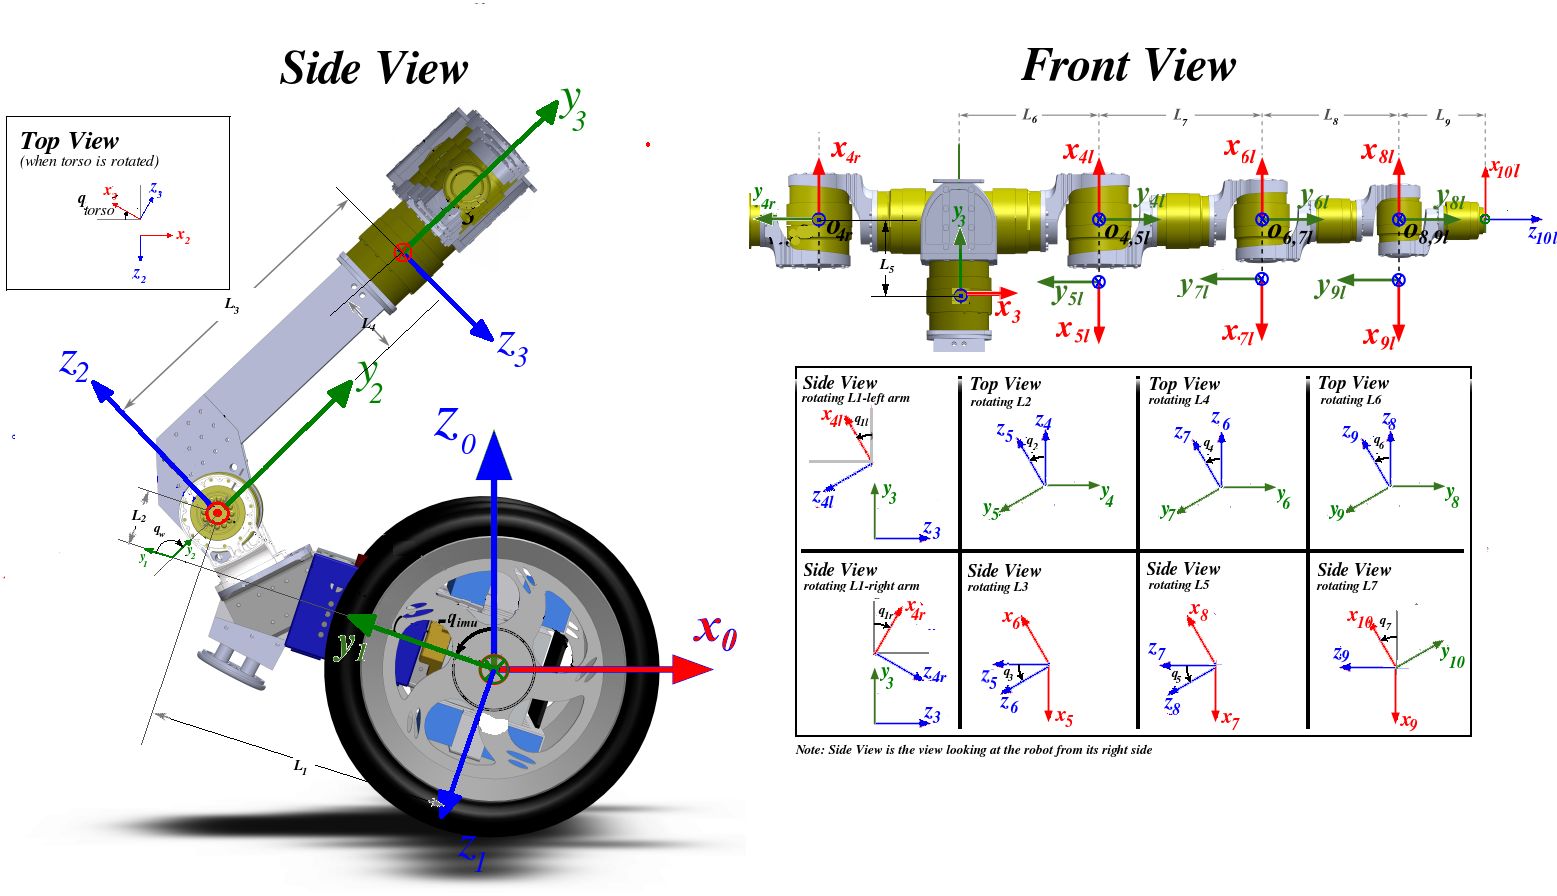
\includegraphics[width=1.0\textwidth]{Figures/framesLHRule.png}
 \caption{Frames of references on the robot}
 \label{fig:frames}
\end{figure}

We will be using the Kane's formulation. This is done so that our current analysis can easily be merged with
the dynamic modelling of wheeled inverted pendulum which is found in terms of quasi-velocities, that prohibit
the use of Lagrange for analytical modelling of the robot. Kane's method however is applicable for this
problem.

\section{Introduction to Kane's Formulation}
\begin{align}
 \sum_{\substack{k}} \left[ m_k \bar{a}_{Gk} \cdot \left(\bar{v}_{Gk}\right)_j + \left( \frac{d\bar{H}_{Gk}}{dt} 
 \right) \cdot \left( \bar\omega_k \right)_j \right] = \sum_{\substack{n}}  \bar{F}_n \cdot \left( \bar{v}_n \right)_j 
 + \sum_{\substack{n}}  \bar{M}_m \cdot \left( \bar{\omega}_m \right)_j \;\; j=1 ... K \label{kanes}
\end{align}
where 
\begin{itemize}[label={}]
\item[$j$] is the unique number identifying each generalized co-ordinate in the system
\item[$k$] is the unique number identifying each rigid body in the system
\item[$n$] is the unique number identifying each external force acting on the system
\item[$m$] is the unique number identifying each external torque acting on the system
\item[$m_k$] is the mass of the $k$th body
\item[$\bar{a}_{Gk}$] is the acceleration of the center of mass of $k$th body
\item[$\bar{v}_{Gk}$] is the velocity of the center of mass of the $k$th body
\item[$\bar{H}_{Gk}$] is the angular momentum of body $k$ about its center of mass
\item[$\bar{\omega}_{k}$] is the angular velocity of the body $k$
\item[$F_n$] is the $n$th external force
\item[$M_m$] is the $m$th external moment
\item[$\bar{v}_{n}$] is the velocity of the point at which external Force $F_n$ is acting
\item[$\bar{\omega}_{m}$] is the angular velocity of the body on which torque is acting relative to the actuator applying the torque
\item[$()_j$] $=\frac{\partial ()}{\partial \dot{q}_j}$ the partial derivative of the quantity in brackets $()$ with respect to the generalized
velocity $\dot{q}_j$
\end{itemize}

\section{Transformations}

The transformation of frame $R_i$ into frame $R_j$ is represented by the homogeneous transformation matrix
${}^{i}T_j$ such that.
\begin{align}
 {}^{i}T_j = \left[\begin{matrix}{}^{i}s_j & {}^{i}n_j & {}^{i}a_j & {}^{i}P_j \end{matrix} \right] 
  = \left[\begin{matrix} & {}^iA_j & & {}^iP_j \\ 0 & 0 & 0 & 1 \end{matrix}\right]
  = \left[\begin{matrix}s_x & n_x & a_x & P_x  \\ s_y & n_y & a_y & P_y 
  \\ s_z & n_z & a_z & P_z \\ 0 & 0 & 0 & 1 \end{matrix} \right]
\end{align}
where ${}^is_j$, ${}^in_j$ and ${}^ia_j$ contain the components of the unit vectors along the $x_j$, 
$y_j$ and $z_j$ axes respectively expressed in frame $R_i$, and where ${}^iP_j$ is the vector representing
the coordinates of the origin of frame $R_j$ expressed in frame $R_i$.

The transformation matrix ${}^iT_j$ can be interpreted as: (a) the transformation from frame $R_i$ to frame $R_j$
and (b) the representation of frame $R_j$ with respect to frame $R_i$. Using figure \ref{fig:frames}, we can
write down these transformation matrices for our system as follows:

\[
 \scalemath{0.75}{{}^0T_1 = \left[\begin{matrix} 0 & sq_{imu} & -cq_{imu} & 0 \\ -1 & 0 & 0 & 0 \\ 0 & cq_{imu} & sq_{imu} & 0 \\ 0 & 0 & 0 & 1 \end{matrix}\right],
 {}^1T_2 = \left[\begin{matrix} 1 & 0 & 0 & 0 \\ 0 & cq_w & sq_w & L_1 \\ 0 & -sq_w & cq_w & -L_2 \\ 0 & 0 & 0 & 1 \end{matrix}\right], 
 {}^2T_3 = \left[\begin{matrix} -cq_{torso} & 0 & sq_{torso} & 0 \\ 0 & 1 & 0 & L_3 \\ -sq_{torso} & 0 & -cq_{torso} & L_4 \\ 0 & 0 & 0 & 1 \end{matrix}\right],}
\]

\[
 \scalemath{0.75}{{}^3T_{4l} = \left[\begin{matrix} 0 & 1 & 0 & L_6 \\ cq_{1l} & 0 & -sq_{1l} & L_5 \\ -sq_{1l} & 0 & -cq_{1l} & 0 \\ 0 & 0 & 0 & 1 \end{matrix}\right], 
 {}^3T_{4r} = \left[\begin{matrix} 0 & -1 & 0 & -L_6 \\ cq_{1r} & 0 & -sq_{1r} & L_5 \\ sq_{1r} & 0 & cq_{1r} & 0 \\ 0 & 0 & 0 & 1 \end{matrix}\right], 
 {}^4T_5 = \left[\begin{matrix} -1 & 0 & 0 & 0 \\ 0 & -cq_2 & -sq_2 & 0 \\ 0 & -sq_2 & cq_2 & 0 \\ 0 & 0 & 0 & 1 \end{matrix}\right], }
\]
 
\[
 \scalemath{0.75}{ {}^5T_6 = \left[\begin{matrix} -cq_3 & 0 & sq_3 & 0 \\ 0 & -1 & 0 & -L_7 \\ sq_3 & 0 & cq_3 & 0 \\ 0 & 0 & 0 & 1 \end{matrix}\right], 
 {}^6T_7 = \left[\begin{matrix} -1 & 0 & 0 & 0 \\ 0 & -cq_4 & -sq_4 & 0 \\ 0 & -sq_4 & cq_4 & 0 \\ 0 & 0 & 0 & 1 \end{matrix}\right], 
 {}^7T_8 = \left[\begin{matrix} -cq_5 & 0 & sq_5 & 0 \\ 0 & -1 & 0 & -L_8 \\ sq_5 & 0 & cq_5 & 0 \\ 0 & 0 & 0 & 1 \end{matrix}\right], }
\]
 
\[
 \scalemath{0.75}{{}^8T_9 = \left[\begin{matrix} -1 & 0 & 0 & 0 \\ 0 & -cq_6 & -sq_6 & 0 \\ 0 & -sq_6 & cq_6 & 0 \\ 0 & 0 & 0 & 1 \end{matrix}\right], 
 {}^9T_{10} = \left[\begin{matrix} -cq_7 & -sq_7 & 0 & 0 \\ 0 & 0 & -1 & -L_9 \\ sq_7 & -cq_7 & 0 & 0 \\ 0 & 0 & 0 & 1 \end{matrix}\right] }
\]


\section{Velocities and Accelerations of Frames}
The angular and linear velocities of the frames can be calculated using the recursive formulation:

\begin{align}
 &{}^j\omega_j={}^jA_i{}^i\omega_i+\dot{q}_j\;{}^je_j \label{recursiveAngVel}\\
 &{}^j\alpha_j={}^jA_i{}^i\alpha_i+\ddot{q}_j\;{}^je_j+\dot{q}_j\;({}^j\omega_j \times {}^je_j) \label{recursiveAngAcc}\\
 &{}^jV_j={}^jA_i\left({}^iV_i+{}^i\omega_i \times {}^iP_j\right) \label{recursiveLinVel}\\
 &{}^ja_j={}^jA_i\left({}^ia_i+{}^i\alpha_i \times {}^iP_j + {}^i\omega_i \times ({}^i\omega_i \times {}^iP_j)\right) \label{recursiveLinAcc}
\end{align} where ${}^i\omega_j$, ${}^i\alpha_j$, ${}^ia_j$ and ${}^iV_j$ denote the angular velocity, linear velocity, 
angular acceleration and linear acceleration repectively of frame $j$ measured with respect to the 
world frame and represented in frame $i$. ${}^je_j$ denotes the direction of local angular velocity of frame $j$ represented in frame $j$. 
$i, j \in \mathbb{F}$ identify the frames and $i$ identifies the antecedent frame of $j$. So, the rotation ${}^jA_i$ and the 
translation ${}^jP_i$ that appear in these equations can not be directly deduced from the transformations listed in the previous section, 
as the they all represent ${}^iT_j$ (note the position of $i$ and $j$). Rather, we need to use following expressions to deduce our matrices:
\begin{align}
 &{}^jA_i = {}^iA_j^T \nonumber \\ 
 &{}^jP_i = -{}^iA_j^T\,{}^iP_j \nonumber
\end{align}

Since frame $R_0$ is fixed ${}^0\omega_0$ and ${}^0V_0$ are both $\left[\begin{matrix}0 & 0 & 0\end{matrix}\right]^T$. We can deduce directions of 
local angular velocities of the frames using figure \ref{fig:frames} as follows.

\[
\scalemath{0.75}{{}^1e_1 = \left[\begin{matrix}-1 & 0 & 0\end{matrix}\right]^T, 
{}^2e_2 = \left[\begin{matrix}-1 & 0 & 0\end{matrix}\right]^T, 
{}^3e_3 = \left[\begin{matrix}0 & -1 & 0\end{matrix}\right]^T, 
{}^4e_4 = \left[\begin{matrix}0 & -1 & 0\end{matrix}\right]^T,}
\]
\[
\scalemath{0.75}{{}^5e_5 = \left[\begin{matrix}-1 & 0 & 0\end{matrix}\right]^T, 
{}^6e_6 = \left[\begin{matrix}0 & -1 & 0\end{matrix}\right]^T, 
{}^7e_7 = \left[\begin{matrix}-1 & 0 & 0\end{matrix}\right]^T, 
{}^8e_8 = \left[\begin{matrix}0 & -1 & 0\end{matrix}\right]^T,}
\]
\[
\scalemath{0.75}{{}^9e_9 = \left[\begin{matrix}-1 & 0 & 0\end{matrix}\right]^T, 
{}^{10}e_{10} = \left[\begin{matrix}0 & 0 & -1\end{matrix}\right]^T}
\]

This information can now be used to derive expressions for the velocities and accelerations of the frames.

\section{Kane's Left-Hand Side}
The inertial forces i.e. the term inside the brackets on the LHS in Kane's formulation can be simplified by expansion
and manipulation that results in cancelation of terms leading to a simplified expression. We show the details of this
manipulation here. The final expression is the outcome in the end which we will use in our code to find the
dynamic model.

\begin{align}
 \scalemath{0.775}{\bar{v}_{Gk}}&\scalemath{0.775}{=\bar{v}_k+\bar{\omega}_k \times \bar{S}_k} \\
 \scalemath{0.775}{\bar{a}_{Gk}}&\scalemath{0.775}{=\bar{a}_k+\bar{\alpha}_k \times \bar{S}_k + \bar{\omega}_k \times (\bar{\omega}_k \times \bar{S}_k)} \label{aGk} \\
 \scalemath{0.775}{\bar{H}_{Gk}}&\scalemath{0.775}{=\mathbf{J}_{Gk} \bar{\omega}_k} \\ 
 \scalemath{0.775}{\frac{d\bar{H}_{Gk}}{dt}}&\scalemath{0.775}{=\mathbf{J}_{Gk} \bar{\alpha}_k + \bar{\omega}_k \times \mathbf{J}_{Gk} \bar{\omega}_k} \nonumber \\
 &\scalemath{0.775}{=(\mathbf{J}_{k}+m_k\mathbf{S}^{\times}_k\mathbf{S}^{\times}_k) \bar{\alpha}_k + \bar{\omega}_k \times (\mathbf{J}_{k}+m_k\mathbf{S}^{\times}_k\mathbf{S}^{\times}_k) \bar{\omega}_k} \nonumber \\
 &\scalemath{0.775}{=\mathbf{J}_{k} \bar{\alpha}_k + \bar{\omega}_k \times \mathbf{J}_{k} \bar{\omega}_k + m_k\mathbf{S}^{\times}_k\mathbf{S}^{\times}_k\bar{\alpha}_k + \bar{\omega}_k \times (m_k\mathbf{S}^{\times}_k\mathbf{S}^{\times}_k \bar{\omega}_k)} \\
 \scalemath{0.775}{m_k \bar{a}_{Gk} \cdot \left(\bar{v}_{Gk}\right)_j} &\scalemath{0.775}{=  m_k \bar{a}_{Gk} \cdot \left(\bar{v}_k+\bar{\omega}_k \times \bar{S}_k\right)_j} \nonumber \\
 &\scalemath{0.775}{=  m_k \bar{a}_{Gk} \cdot \left(\bar{v}_k\right)_j + m_k \bar{a}_{Gk} \cdot \left(\bar{\omega}_k \times \bar{S}_k\right)_j} \nonumber \\
 &\scalemath{0.775}{=  m_k \bar{a}_{Gk} \cdot \left(\bar{v}_k\right)_j - m_k \left( \bar{a}_k+\bar{\alpha}_k \times \bar{S}_k + \bar{\omega}_k \times (\bar{\omega}_k \times \bar{S}_k) \right) \cdot \left(\bar{S}_k \times \bar{\omega}_k\right)_j} \nonumber \\
 &\scalemath{0.775}{=  m_k \bar{a}_{Gk} \cdot \left(\bar{v}_k\right)_j - m_k \left( \bar{a}_k-\bar{S}_k \times \bar{\alpha}_k - \bar{\omega}_k \times (\bar{S}_k \times \bar{\omega}_k) \right) \cdot \left(\bar{S}_k \times \left(\bar{\omega}_k\right)_j\right)} \nonumber \\
 &\scalemath{0.775}{=  m_k \bar{a}_{Gk} \cdot \left(\bar{v}_k\right)_j - m_k \left( \bar{a}_k-\mathbf{S}^{\times}_k \bar{\alpha}_k - \mathbf{\omega}^{\times}_k \mathbf{S}^{\times}_k \bar{\omega}_k \right)^T  \mathbf{S}^{\times}_k \left(\bar{\omega}_k\right)_j} \nonumber \\
 &\scalemath{0.775}{=  m_k \bar{a}_{Gk} \cdot \left(\bar{v}_k\right)_j - m_k \left( \mathbf{S}^{\times T}_k \bar{a}_k -  \mathbf{S}^{\times T}_k \mathbf{S}^{\times}_k \bar{\alpha}_k - \mathbf{S}^{\times T}_k \mathbf{\omega}^{\times}_k \mathbf{S}^{\times}_k \bar{\omega}_k \right)^T  \left(\bar{\omega}_k\right)_j} \nonumber \\
 &\scalemath{0.775}{=  m_k \bar{a}_{Gk} \cdot \left(\bar{v}_k\right)_j + m_k \left( \mathbf{S}^{\times}_k \bar{a}_k -  \mathbf{S}^{\times}_k \mathbf{S}^{\times}_k \bar{\alpha}_k - \mathbf{S}^{\times}_k \mathbf{\omega}^{\times}_k \mathbf{S}^{\times}_k \bar{\omega}_k \right)^T  \left(\bar{\omega}_k\right)_j} \nonumber \\
 &\scalemath{0.775}{=  m_k \bar{a}_{Gk} \cdot \left(\bar{v}_k\right)_j + m_k \left( \bar{S}_k \times \bar{a}_k -  \bar{S}_k \times \bar{S}_k \times \bar{\alpha}_k - \bar{S}_k \times ( \bar{\omega}_k \times ( \bar{S}_k \times \bar{\omega}_k ) ) \right) \cdot  \left(\bar{\omega}_k\right)_j} \nonumber \\
 &\scalemath{0.775}{=  m_k \bar{a}_{Gk} \cdot \left(\bar{v}_k\right)_j + m_k \left( \bar{S}_k \times \bar{a}_k -  \bar{S}_k \times \bar{S}_k \times \bar{\alpha}_k + \bar{\omega}_k \times ( ( \bar{S}_k \times \bar{\omega}_k ) \times  \bar{S}_k ) + ( \bar{S}_k \times \bar{\omega}_k ) \times ( \bar{S}_k \times \bar{\omega}_k )  \right) \cdot  \left(\bar{\omega}_k\right)_j} \nonumber \\
 &\scalemath{0.775}{=  m_k \bar{a}_{Gk} \cdot \left(\bar{v}_k\right)_j + m_k \left( \bar{S}_k \times \bar{a}_k -  \bar{S}_k \times \bar{S}_k \times \bar{\alpha}_k - \bar{\omega}_k \times ( \bar{S}_k \times ( \bar{S}_k \times \bar{\omega}_k ) ) + 0  \right) \cdot  \left(\bar{\omega}_k\right)_j} \nonumber \\
 &\scalemath{0.775}{=  m_k \bar{a}_{Gk} \cdot \left(\bar{v}_k\right)_j + \left( m_k \bar{S}_k \times \bar{a}_k -  m_k \mathbf{S}^{\times}_k \mathbf{S}^{\times}_k \bar{\alpha}_k - \bar{\omega}_k \times (m_k \mathbf{S}^{\times}_k \mathbf{S}^{\times}_k \bar{\omega}_k) \right) \cdot  \left(\bar{\omega}_k\right)_j} \\
 \scalemath{0.775}{m_k \bar{a}_{Gk} \cdot \left(\bar{v}_{Gk}\right)_j} &\scalemath{0.775}{ + \left( \frac{d\bar{H}_{Gk}}{dt} \right) \cdot \left( \bar\omega_k \right)_j} \nonumber \\
 &\scalemath{0.775}{=  m_k \bar{a}_{Gk} \cdot \left(\bar{v}_k\right)_j + \left( m_k \bar{S}_k \times \bar{a}_k -  m_k \mathbf{S}^{\times}_k \mathbf{S}^{\times}_k \bar{\alpha}_k - \bar{\omega}_k \times (m_k \mathbf{S}^{\times}_k \mathbf{S}^{\times}_k \bar{\omega}_k) \right) \cdot  \left(\bar{\omega}_k\right)_j} \nonumber \\
 &\scalemath{0.775}{\hspace{40pt}+\left(\mathbf{J}_{k} \bar{\alpha}_k + \bar{\omega}_k \times \mathbf{J}_{k} \bar{\omega}_k + m_k\mathbf{S}^{\times}_k\mathbf{S}^{\times}_k\bar{\alpha}_k + \bar{\omega}_k \times (m_k\mathbf{S}^{\times}_k\mathbf{S}^{\times}_k \bar{\omega}_k)\right) \cdot \left( \bar\omega_k \right)_j} \nonumber \\
 &\scalemath{0.775}{=  m_k \bar{a}_{Gk} \cdot \left(\bar{v}_k\right)_j + \left( m_k \bar{S}_k \times \bar{a}_k + \mathbf{J}_{k} \bar{\alpha}_k + \bar{\omega}_k \times \mathbf{J}_{k} \bar{\omega}_k\right) \cdot  \left(\bar{\omega}_k\right)_j} \label{kanesLHSTerm}
\end{align}

The terms $\bar\omega_k$, $\bar\alpha_k$, $\bar{v}_k$, $\bar{a}_k$ will be found using the recursive formulations in eqs. \ref{recursiveAngVel}-\ref{recursiveLinAcc}. And the 
term $\bar{a}_{Gk}$ will be found using eq.\ref{aGk}. $\scalemath{0.75}{\bar{S}_k=\left[\begin{matrix} \mathbf{X}_k & \mathbf{Y}_k & \mathbf{Z}_k \end{matrix}\right]^T}$ 
is the center of mass of the joint represented in the local frame. We will use the symbol $\mathbf{MS}_k$ to represent mass times center of mass ($m_k\mathbf{S}_k$) which is
the vector the components of which are $\scalemath{0.75}{\mathbf{MS}=\left[\begin{matrix} \mathbf{MX} & \mathbf{MY} & \mathbf{MZ} \end{matrix}\right]^T}$. 
Finally, $\scalemath{0.75}{\mathbf{J}_k=\left[\begin{matrix} \mathbf{XX}_k & \mathbf{XY}_k & \mathbf{XZ}_k \\ \mathbf{XY}_k & \mathbf{YY}_k & \mathbf{YZ}_k \\ \mathbf{XZ}_k & \mathbf{YZ}_k & \mathbf{ZZ}_k \end{matrix}\right]}$
is the inertia matrix of the joint represented in the local frame.

\section{Kane's Right-Hand Side}
The right hand side of the Kane's forumulation \ref{kanes} is the sum of some dot product terms. Each term is either the
dot product of:
\begin{itemize}
 \item force applied on the system $\bar{F}_n$
 \item the linear velocity $\bar{v}_n$ of the point differentiated partially wrt the the unique gerneralized speed 
 $\dot{q}_j$ corresponding to each equation i.e. $\frac{\partial \bar{v}_n}{\partial \dot{q}_j}$\\
\end{itemize}
or the dot product of:
\begin{itemize}
 \item torque applied on the system $\bar{\tau}_n$
 \item the angular velocity $\bar{\omega}_n$ of the body differentiated partially wrt the the unique gerneralized speed 
 $\dot{q}_j$ corresponding to each equation i.e. $\frac{\partial \bar{\omega}_n}{\partial \dot{q}_j}$
\end{itemize}

So, in order to analyse the right-hand side of the equation, we need to list down all the forces and torques applied
to the system and the points at which they are being applied. They are as follows. 
\begin{itemize}[label={}]
 \item[$\bar\tau_j$] $=\tau_j\bar{e}_j$ The torque applied by each joint motor fixed on the antecedent joint moving the current joint. There
 are 17 such torques as \[ \tau_j \in \{ \tau_{imu}, \tau_{w}, \tau_{torso}, \tau_{1l}, ... , \tau_{7l}, \tau_{1r}, ... , \tau_{7r} \} \]
 Note that $\tau_{imu} = -\tau_R-\tau_L$ where $\tau_R$ and $\tau_L$ are torques applied to the right and left wheel respectively,
 and $\tau_{imu}$ is the sum of reactions torques experienced by the base in response.
 \item[$-\bar\tau_j$] $=-\tau_j\bar{e}_j$ The reaction torque experienced by each antecedent joint.
 \item[$\bar{F}_{gk}$] $=m_k\bar{g}$ is the weight of each joint $k$
 \item[$\bar{F}_{el}, \bar{\tau}_{el}$] Force and torque applied by the environment on the left hand end-effector at point $E_l$
 \item[$\bar{F}_{er}, \bar{\tau}_{er}$] Force and torque applied by the environment on the right hand end-effector at point $E_r$
\end{itemize}
\subsection{Joint Torques}
The contribution of motor torque of joint $k$ and its reaction, on the right-hand side of Kane's equation corresponding to generalized speed 
$\dot{q}_j$ is: 
\begin{align}
 &\tau_k\bar{e}_k \cdot \frac{\partial \bar\omega_k}{\partial \dot{q}_j} - \tau_k\bar{e}_k \cdot \frac{\partial \bar\omega_{a(k)}}{\partial \dot{q}_j} \label{jointTorque1}
\end{align}
where $a(k) =$ antecedent frame of $k$. The first term is the contribution of action torques and the second term is the contribution
of the reaction torques.
Since
\begin{align}
 \bar\omega_k &= \dot{q}_1\bar{e}_1 + \dot{q}_2\bar{e}_1 + \dot{q}_3\bar{e}_3 + ... + \dot{q}_k\bar{e}_k \nonumber \\
 \frac{\partial \bar\omega_k}{\partial \dot{q}_j} &= \begin{cases}
                                                      0         & \mbox{if } k < j \\
                                                      \bar{e}_j & \mbox{if } k \geq j 
                                                     \end{cases} \label{diffOmega}
\end{align}
If we take the summation of all joint torque contibutions each described by expression \ref{jointTorque1} i.e. for $k=1...K$, 
to get get the right-hand side contribution by all joint torques in the kane's equaiton corresponding to a generalized speed $j$, 
we will get a very simplified solution
\begin{align}
  \sum\limits_{k=1}^K &\left( \tau_k\bar{e}_k \cdot \frac{\partial \bar\omega_k}{\partial \dot{q}_j} - \tau_k\bar{e}_k \cdot \frac{\partial \bar\omega_{k-1}}{\partial \dot{q}_j} \right) \nonumber \\   
 &= \sum\limits_{k=1}^{j-1} \left(          \tau_k\bar{e}_k \cdot \frac{\partial \bar\omega_k}{\partial \dot{q}_j} - \tau_k\bar{e}_k \cdot \frac{\partial \bar\omega_{k-1}}{\partial \dot{q}_j}\right) \nonumber \\
      &\;\;\;+                              \tau_j\bar{e}_j \cdot \frac{\partial \bar\omega_j}{\partial \dot{q}_j} - \tau_j\bar{e}_j \cdot \frac{\partial \bar\omega_{j-1}}{\partial \dot{q}_j} \nonumber \\
      &\;\;\;+ \sum\limits_{k=j+1}^K \left( \tau_k\bar{e}_k \cdot \frac{\partial \bar\omega_k}{\partial \dot{q}_j} - \tau_k\bar{e}_k \cdot \frac{\partial \bar\omega_{k-1}}{\partial \dot{q}_j} \right) \nonumber \\
 &= \sum\limits_{k=1}^{j-1} \left(   0 - 0 \right) + \tau_j\bar{e}_j \cdot \bar{e}_j - 0 + \sum\limits_{k=j+1}^K \left( \tau_k\bar{e}_k \cdot \bar{e}_j - \tau_k\bar{e}_k \cdot \bar{e}_j \right) \nonumber \\
 &= \tau_j \label{jointTorque2}
\end{align}

So the total joint torques contributions on the RHS of each Kane's equation is just the joint torque actuating the generalized speed wrt
which the equaiton is being evaluated.

\subsection{End-effector Forces and Torques}
Let $\bar{F}_{e}$ and $\bar\tau_{e}$ be the force and torque being applied by the environment on the end-effector. The contribution on the 
RHS of Kane's equaiton corresponding to generalized speed $\dot{q}_j$ will be:
\begin{align}
 \bar{F}_{e} \cdot \frac{\partial \bar{v}_e}{\partial \dot{q}_j} + \bar\tau_{e} \cdot \frac{\partial \bar\omega_K}{\partial \dot{q}_j} \label{endEff1}
\end{align}
where $\bar{v}_e$ is the linear velocity of the point $E$ on the end-effector on which the force is being applied. And $\bar\omega_K$ is the angular velocity
of the last joint on which the end-effector is mounted.
\begin{align}
 \bar{v}_e &= \bar{v}_K + \bar\omega_K \times \bar{r}_{e/O_{K}} \nonumber \\
 &= \bar{v}_{K-1} + \bar\omega_{K-1} \times \bar{r}_{O_{K}/O_{K-1}} + \bar\omega_K \times \bar{r}_{E/O_{K}} \nonumber \\
 &...  \nonumber \\
 &= \bar{v}_0 + \bar\omega_0 \times \bar{r}_{O_1/O_0} + \bar\omega_1 \times \bar{r}_{O_2/O_1} + \bar\omega_2 \times \bar{r}_{O_3/O_2} + ... + \bar\omega_{K-1} \times \bar{r}_{O_{K}/O_{K-1}} + \bar\omega_K \times \bar{r}_{O_{K+1}/O_{K}} \nonumber \\
 &= \bar{v}_0 + \sum\limits_{k=0}^K \left( \bar\omega_k \times \bar{r}_{O_{k+1}/O_k} \right)
\end{align}
where we have replace $E$ with $O_{K+1}$ for the convenience of writing the closed-form expression. When partially differentiated wrt $\dot{q}_j$ 
we can use eq. \ref{diffOmega} to get:
\begin{align}
 \frac{\partial \bar{v}_e}{\partial \dot{q}_j} &= \frac{\partial \bar{v}_0}{\partial \dot{q}_j} + \sum\limits_{k=0}^K \left( \frac{\partial \bar\omega_k}{\partial \dot{q}_j} \times \bar{r}_{O_{k+1}/O_k} \right) \nonumber \\
 &= 0 + \sum\limits_{k=0}^{j-1} \left( \frac{\partial \bar\omega_k}{\partial \dot{q}_j} \times \bar{r}_{O_{k+1}/O_k} \right) 
       + \sum\limits_{k=j}^K \left( \frac{\partial \bar\omega_k}{\partial \dot{q}_j} \times \bar{r}_{O_{k+1}/O_k} \right) \nonumber \\
 &= \sum\limits_{k=0}^{j-1} \left( 0 \times \bar{r}_{O_{k+1}/O_k} \right) + \sum\limits_{k=j}^K \left( \bar{e}_j \times \bar{r}_{O_{k+1}/O_k} \right) \nonumber \\
 &= \bar{e}_j \times \sum\limits_{k=j}^K \bar{r}_{O_{k+1}/O_k} \nonumber \\
 &= \bar{e}_j \times \left( \bar{r}_{O_{j+1}/O_j} + \bar{r}_{O_{j+2}/O_{j+1}} + \bar{r}_{O_{j+3}/O_{j+2}} + ... + \bar{r}_{O_{K+1}/O_K}\right) \nonumber \\
 &= \bar{e}_j \times \bar{r}_{O_{K+1}/O_j} \nonumber \\
 &= \bar{e}_j \times \bar{r}_{E/O_j} \label{diffVe}
\end{align}
Substituting eqs. \ref{diffVe} and \ref{diffOmega} in expression \ref{endEff1}, we get
\begin{align}
 &\bar{F}_{e} \cdot \bar{e}_j \times \bar{r}_{E/O_j} + \bar\tau_{e} \cdot \bar{e}_j \nonumber \\
 &= \left[\begin{matrix} \left[\bar{e}_j \times \bar{r}_{E/O_j}\right]^T & \bar{e}_j^T \end{matrix} \right]\left[\begin{matrix} \bar{F}_e \\ \bar{\tau}_e \end{matrix} \right] \nonumber 
\end{align}
If we write all kane's equations in the form of a vector then the right hand side contribution of end-effector force and torque will become,
\begin{align}
 &\left[\begin{matrix}
 \left[\bar{e}_1 \times \bar{r}_{E/O_1}\right]^T & \bar{e}_1^T  \\
 \left[\bar{e}_2 \times \bar{r}_{E/O_2}\right]^T & \bar{e}_2^T  \\
 \left[\bar{e}_3 \times \bar{r}_{E/O_3}\right]^T & \bar{e}_3^T  \\
 ... & \\
 \left[\bar{e}_K \times \bar{r}_{E/O_K}\right]^T & \bar{e}_K^T  \\ 
 \end{matrix} \right]
 \left[\begin{matrix} \bar{F}_e \\ \bar{\tau}_e \end{matrix} \right] \nonumber \\ 
 &= \mathbb{J}^T\mathbbm{f}_e \label{endEff2}
\end{align}
where
\begin{align}
 \mathbb{J} &= \left[\begin{matrix} \bar{e}_1 \times \bar{r}_{E/O_1} & ... & \bar{e}_K \times \bar{r}_{E/O_K} \\ \bar{e}_1 & ... & \bar{e}_K\end{matrix} \right] \nonumber \\
 \mathbbm{f} &= \left[\begin{matrix} \bar{F}_e \\ \bar{\tau}_e \end{matrix} \right] \nonumber
\end{align}

The matrix $\mathbb{J}$ is refered to as the Jacobian. And $\mathbbm{f}$ is the wrench (formal term to
refer to a force/torque couple). This whole theory was assuming a single serial chain of the robot with a single
end-effector. For the case of krang, we will have two wrenches $\mathbbm{f}_{el}$ and $\mathbbm{f}_{er}$ applied at 
two end-effectors on the right and the left arms respectively. The points on which this wrench is being sensed
on the two end-effectors is $E_L$ and $E_R$. So the contribution becomes:
\begin{align}
 \mathbb{J}_{L}^T\mathbbm{f}_{el} + \mathbb{J}_{R}^T\mathbbm{f}_{er}
\end{align} where
\begin{itemize}
 \item $\scalemath{0.775}{\mathbb{J}_{L} = \left[ \begin{matrix} e_1\times \bar{r}_{E_L/O_1} & e_2\times \bar{r}_{E_L/O_2} 
 & e_3\times \bar{r}_{E_L/O_3} & e_{4l}\times \bar{r}_{E_L/O_{4l}} & ... & e_{10l}\times \bar{r}_{E_L/O_{10l}} & O_{3\times 7} \\ 
 e_1 & e_2 & e_3 & e_{4l} & ... & e_{10l} & O_{3\times 7} \end{matrix} \right]}$
 \item $\scalemath{0.75}{\mathbb{J}_{10r} = \left[ \begin{matrix} e_1\times \bar{r}_{E_R/O_1} & e_2\times \bar{r}_{E_R/O_2} 
 & e_3\times \bar{r}_{E_R/O_3} & O_{3\times 7} & e_{4r}\times \bar{r}_{E_R/O_{4r}} & ... & e_{10r}\times \bar{r}_{E_R/O_{10r}} \\ 
 e_1 & e_2 & e_3 & O_{3\times 7} & e_{4r} & ... & e_{10r}  \end{matrix} \right]}$
\end{itemize}

\subsection{Gravitational Forces}
The contribution of the weight of a joint $k$ to the right-hand side of the equation corresponding to generalized speed
$\dot{q}_j$ is
\begin{align}
 &m_k\bar{g} \cdot \frac{\partial \bar{v}_{Gk}}{\partial \dot{q}_j} \label{gravity1}
\end{align}
Now
\begin{align}
 \bar{v}_{Gk} &= \bar{v}_k + \bar\omega_k \times \bar{r}_{Gk/O_k} \nonumber \\
 &= \bar{v}_{k-1} + \bar\omega_{k-1} \times r_{O_{k}/O_{k-1}} + \bar\omega_k \times \bar{r}_{Gk/O_k} \nonumber \\
 &= \bar{v}_0 + \sum\limits_{i=1}^{k} \left( \bar\omega_{i-1} \times r_{O_{i}/O_{i-1}} \right) + \bar\omega_k \times \bar{r}_{Gk/O_k}  \nonumber \\ 
 \frac{\partial \bar{v}_{Gk}}{\partial \dot{q}_j} &= \frac{\partial \bar{v}_0}{\partial \dot{q}_j} + \sum\limits_{i=1}^{k} \left( \frac{\partial \bar\omega_{i-1}}{\partial \dot{q}_j} \times r_{O_{i}/O_{i-1}} \right) + \frac{\partial \bar\omega_k}{\partial \dot{q}_j} \times \bar{r}_{Gk/O_k}  \nonumber \\ 
 &= 0 + \sum\limits_{i=1}^{k} \left( \frac{\partial \bar\omega_{i-1}}{\partial \dot{q}_j} \times r_{O_{i}/O_{i-1}} \right) + \frac{\partial \bar\omega_k}{\partial \dot{q}_j} \times \bar{r}_{Gk/O_k}  \nonumber \\
 &= \begin{cases}
     0 & \mbox{if } k < j \\
     \sum\limits_{i=j+1}^{k} \left( \bar{e}_j \times r_{O_{i}/O_{i-1}} \right) + \bar{e}_j \times \bar{r}_{Gk/O_k} & \mbox{if } k \geq j
    \end{cases} \nonumber \\
 &= \begin{cases}
     0 & \mbox{if } k < j \\
     \bar{e}_j \times \left( \sum\limits_{i=j+1}^{k} \bar{r}_{O_{i}/O_{i-1}} + \bar{r}_{Gk/O_k}\right) & \mbox{if } k \geq j
    \end{cases} \nonumber \\
 &= \begin{cases}
     0 & \mbox{if } k < j \\
     \bar{e}_j \times \bar{r}_{Gk/O_j} & \mbox{if } k \geq j
    \end{cases} 
\end{align}
The total contributions of all joints will therefore be:
\begin{align}
 &\sum\limits_{k=1}^K \left( m_k\bar{g} \cdot \frac{\partial \bar{v}_{Gk}}{\partial \dot{q}_j} \right) \nonumber \\
 &= \bar{g} \cdot \left( \sum\limits_{k=1}^{j-1} m_k\frac{\partial \bar{v}_{Gk}}{\partial \dot{q}_j} + \sum\limits_{k=j}^{K} m_k\frac{\partial \bar{v}_{Gk}}{\partial \dot{q}_j} \right) \nonumber \\ 
 &= \bar{g} \cdot \left( \sum\limits_{k=1}^{j-1} 0 + \sum\limits_{k=j}^{K} m_k\left({e}_j \times \bar{r}_{Gk/O_j} \right) \right) \nonumber \\
 &= \bar{g} \cdot \left( {e}_j \times \sum\limits_{k=j}^{K} m_k\bar{r}_{Gk/O_j} \right) \label{gravity2}
\end{align}
Note that this derivation is assuming a single serial chain. In the case of Krang however, if $j$ corresponds to a 
speed of joint before the branching takes place i.e. if $j \in \{ imu, w, torso \}$ the range of summation will include
all joints in the tree above the current joint. If $j$ corresponds to the speed of joint in one of the branches
i.e. if $j \in \{ 1l, ... , 7l \}$ or $j \in \{ 1r, ... , 7r \}$ then the range of summation will only be consisting
of joints following the current joint in the specific branch.

\section{MATLAB code For Finding the Dynamic Model}

The dynamic model is generated using a script \texttt{dynamicModel.m} found in the folder 
\textit{\relsize{-1} stableForceInteraction/Implementation/1-ForceControlWhileBalancing/1-ControlProblem1/1-DynamicModeling/2-DynamicModelOfTreeStructuredRobot/2-matlab/Kanes}.
The function populates the frame information in a map container using \texttt{getKrangFrames()}, then 
calculates the left-hand side of the Kane's terms using the function \texttt{kanesLHS()} and finally
constructs the $\mathbf{A}$ and $\mathbf{C}$ matrices in the dynamic model using the function 
\texttt{getAC()}. These functions and the data structures are briefly discussed in the following
subsections.

\subsection{Map Container for all the Frame Information}

The function \texttt{getKrangFrames()} populates the information in a map container \texttt{f}. A map container is a data structure
in MATLAB that stores a list of data that is retrievable using a key. We store a \texttt{frame} structure in each
cell of the map and use strings $s \in \mathbf{S} = \lbrace$ \texttt{\textquotesingle 0\textquotesingle }, \texttt{\textquotesingle 1\textquotesingle }, 
\texttt{\textquotesingle 2\textquotesingle }, \texttt{\textquotesingle 3\textquotesingle }, \texttt{\textquotesingle 4l\textquotesingle }, 
\texttt{\textquotesingle 5l\textquotesingle }, \texttt{\textquotesingle 6l\textquotesingle }, \texttt{\textquotesingle 7l\textquotesingle },
\texttt{\textquotesingle 8l\textquotesingle }, \texttt{\textquotesingle 9l\textquotesingle }, \texttt{\textquotesingle 10l\textquotesingle },
\texttt{\textquotesingle 4r\textquotesingle }, \texttt{\textquotesingle 5r\textquotesingle }, \texttt{\textquotesingle 6r\textquotesingle }, 
\texttt{\textquotesingle 7r\textquotesingle }, \texttt{\textquotesingle 8r\textquotesingle }, \texttt{\textquotesingle 9r\textquotesingle }, 
\texttt{\textquotesingle 10r\textquotesingle } $\rbrace$ as a key to retrieve information. The \texttt{frame} structure
stores the following elements:
\begin{itemize}[label={}]
 \item[\texttt{x}] the unit vector along $x$-axis represented in the antecedent frame
 \item[\texttt{y}] the unit vector along $y$-axis represented in the antecedent frame
 \item[\texttt{z}] the unit vector along $z$-axis represented in the antecedent frame
 \item[\texttt{P}] the position of the origin frame represented in the antecedent frame
 \item[\texttt{e}] the unit vector along direction of positive rotation of the frame represented in the local frame
 \item[\texttt{a}] the string $\in \mathbf{S}$ (defined above) that is the key that maps to the antecedent frame
 \item[\texttt{q}] the symbolic variable used for representing the generalized position $q$ associated with this frame
 \item[\texttt{dq}] the symbolic variable used for representing the generalized speed $\dot{q}$ associated with this frame
 \item[\texttt{ddq}] the symbolic variable used for representing the generalized acceleration $\ddot{q}$ associated with this frame
 \item[\texttt{o}] the row number in the inertia matrix $\mathbf{A}$ (i.e. in the final dynamic model $\mathbf{A\ddot{q}+C\dot{q}+Q=F}$) 
 that corresponds to the current joint 
 \item[\texttt{param}] array of ten symbolic variables used to represent the inertial parameters of the joint
 $\scalemath{0.75}{\left[\begin{matrix} m & \mathbf{MX} & \mathbf{MY} & \mathbf{MZ} & \mathbf{XX} & \mathbf{YY} & \mathbf{ZZ} & \mathbf{XY} & \mathbf{XZ} & \mathbf{YZ} \end{matrix}\right]^T}$
\end{itemize}

\subsection{Functions associated with the Map Container}

There are a number of functions that take the map container \texttt{f} as the input argument and construct a useful
information as an output. Here is a list of those functions:
\begin{itemize}[label={}]
 \item[\texttt{\relsize{-2} isBefore(f, key1, key2)}] returns \texttt{true} if frame 1 (identified by \texttt{key1}) is before frame 2 
 (identified by \texttt{key2}) in the tree structure of the robot
 \item[\texttt{\relsize{-2} Rot(f, key1, key2)}] returns rotation transform ${}^jA_i$ i.e. represention of frame i (identified by \texttt{key1}) in frame j (identified by \texttt{key2})
 \item[\texttt{\relsize{-2} Tf(f, key1, key2)}] returns rotation transform ${}^jT_i$ i.e. represention of frame i (identified by \texttt{key1}) in frame j (identified by \texttt{key2})
 \item[\texttt{\relsize{-2} qVec(f)}] generates the vector $\mathbf{q}$ containing generalized positions of all frames
 \item[\texttt{\relsize{-2} dqVec(f)}] generates the vector $\mathbf{\dot{q}}$ containing generalized speeds of all frames
 \item[\texttt{\relsize{-2} ddqVec(f)}] generates the vector $\mathbf{\ddot{q}}$ containing generalized accelerations of all frames
 \item[\texttt{\relsize{-2} mass(f, key)}] returns the mass of the frame identified by the \texttt{key}
 \item[\texttt{\relsize{-2} mCOM(f, key)}] returns the mass times COM ($\scalemath{0.75}{\mathbf{MS}=\left[\begin{matrix} \mathbf{MX} & \mathbf{MY} & \mathbf{MZ} \end{matrix}\right]^T}$)
 of the joint identified by the \texttt{key} represented in the local frame
 \item[\texttt{\relsize{-2} inertiaMat(f, key)}] returns the inertia matrix 
 ($\scalemath{0.75}{\mathbf{J}=\left[\begin{matrix} \mathbf{XX} & \mathbf{XY} & \mathbf{XZ} \\ \mathbf{XY} & \mathbf{YY} & \mathbf{YZ} \\ \mathbf{XZ} & \mathbf{YZ} & \mathbf{ZZ} \end{matrix}\right]}$)
 of the joint indentified by \texttt{key} represented in the local frame
 \item[\texttt{\relsize{-2} angVel(f, key)}] returns the symbolic expression for the angular velocity ($\bar\omega$) of the joint represented in local frame calculated
 recursively using eq. \ref{recursiveAngVel}
 \item[\texttt{\relsize{-2} angAcc(f, key)}] returns the symbolic expression for the angular acceleration ($\bar\alpha$) of the joint represented in local frame calculated
 recursively using eq. \ref{recursiveAngAcc}
 \item[\texttt{\relsize{-2} linVel(f, key)}] returns the symbolic expression for the linear velocity ($\bar{v}$) of the joint represented in local frame calculated
 recursively using eq. \ref{recursiveLinVel}
 \item[\texttt{\relsize{-2} linAcc(f, key)}] returns the symbolic expression for the linear acceleration ($\bar{a}$) of the joint represented in local frame calculated
 recursively using eq. \ref{recursiveLinAcc}
\end{itemize}

\subsection{Kane's Left-Hand Side}
Kane's formulation (eq.\ref{kanes}) gives a number of equations, one for each generalized speed $\dot{q}_j$. The left-hand side
of each equation is a summation of a number of terms one for each joint $k$. Each term is calculated using 
eq.\ref{kanesLHSTerm} which gives a simplified version of what occured in the brackets on which the summation
is operating on the left-hand side of the original Kane's equation.

The function \texttt{kanesLHS()} is written to calculate the symbolic expression for the left hand side of each equation.
The function iterates through each joint $k$ using the keys to the map container. For each joint it:
\begin{itemize}
 \item evaluates the symbolic expressions for the respective joint velocities and accelerations ($\bar\omega_k$, $\bar\alpha_k$, 
 $\bar{v}_k$ and $\bar{a}_k$) using the helper functions described in the previous subsection
 \item evaluates for this joint $k$ the symbolic expression for the term in the brackets, on which the summation
 is operating on the left-hand side of the original Kane's equation, using eq.\ref{kanesLHSTerm}. A term
 for each equation with respect to each generalized speed $\dot{q}_j$ (i.e. a  sub-loop iterating through all generalized speeds). 
 This gives the contribution of the inertial forces of joint $k$ to the left-hand side
 of each equation in the Kane's formulation.
 \item adds the final expression to an accumulator (to apply the summation)
\end{itemize}
A vector of size the same as the number of Kane's eqations is thus generated each element of which corresponds to a unique generalized speed $q_j$ and
represents the sum of all joint contributions with respect to the unique joint speed corresponding to this element. So each element represents
the left-hand side of the each equation in the Kane's formulation.

Finally, once all the symbolic expressions are generated using \texttt{kanesLHS()}, we collect the coefficients of each $\ddot{q}_j$
and $\dot{q}_j$ in each equation to generate our $\mathbf{A}$ and $\mathbf{C}$ matrices in the final dynamic equation 
$\mathbf{A\ddot{q}+C\dot{q}+Q=F}$. These matrices are saved in the symbolic variable matrices \texttt{AA} and \texttt{CC}.
These variables can be loaded into the workspace by loading the file \texttt{kanesLHS.mat}.

\subsection{Kane's Right-Hand Side}
The evaluation of right-hand is written in a separate script \texttt{kanesRHS.m}. It uses the original closed form
expressions for the evaluation of the forces i.e. eqs. \ref{jointTorque1}, \ref{endEff1} and \ref{gravity1}. 
The derivation of the simplified expressions presented in eqs. \ref{jointTorque2}, \ref{endEff2} and \ref{gravity2} 
could also be used but we did not use them. We can write a separate code later to verify the results of the former by comparing it with the
result of derived expressions. We have not done that as yet.

The result of the right-hand side evaluation is stored in the symbolic variable vectors \texttt{a, b1, b2, b3, b4 and c}
containing contributions of $\bar\tau_j$, $\bar{F}_{el}$, $\bar\tau_{el}$, $\bar{F}_{er}$, $\bar\tau_{er}$ and
$\bar{F}_{gk}$ respectively. The code can be found in the appendix.


% 
% \section{Potential Energy}
% The total potential energy $U$ of the robot is given by:
% \begin{align}
%  U = \sum_{\substack{j \in \mathbb{F}}} U_j = \sum_{\substack{j \in \mathbb{F}}} -M_j \mathbf{g}^T(L_{0,j}+S_j) \label{eq:PE1}
% \end{align}
% where $L_{0,j}$ is the position vector from the origin $O_0$ to $O_j$ and $\mathbf{g}$ is the gravitatonal acceleration. Projecting 
% the vectors appearing in \ref{eq:PE1} into frame $R_0$, we obtain:
% \begin{align}
%  U_j &= -M_j\,{}^0\mathbf{g}^T({}^0P_j+{}^0A_j\,{}^jS_j) \\ &= -{}^0\mathbf{g}^T(M_j\,{}^0P_j+{}^0A_j\,{}^j\mathbf{MS}_j) \\ 
%  &= -\left[\begin{matrix} {}^0\mathbf{g}^T && 0 \end{matrix} \right] {}^0T_j\left[ \begin{matrix} {}^j\mathbf{MS}_j \\ M_j \end{matrix} \right]
% \end{align}
% Given the frames defined in figure \ref{fig:frames}, ${}^0\mathbf{g} = \left[\begin{matrix}0 & 0 & -g \end{matrix}\right]^T$.
% 
\section{Appendix}

We present the code listings of the various functions in this section.

\subsection{\texttt{dynamicModel.m}}
\lstinputlisting[language=Matlab]{../../2-matlab/Kanes/dynamicModel.m}

\subsection{\texttt{getKrangFrames()}}
\lstinputlisting[language=Matlab]{../../2-matlab/Kanes/getKrangFrames.m}

\subsection{\texttt{kanesLHS()}}
\lstinputlisting[language=Matlab]{../../2-matlab/Kanes/kanesLHS.m}

\subsection{\texttt{getAC()}}
\lstinputlisting[language=Matlab]{../../2-matlab/Kanes/getAC.m}

\subsection{\texttt{angVel()}}
\lstinputlisting[language=Matlab]{../../2-matlab/Kanes/angVel.m}

\subsection{\texttt{angAcc()}}
\lstinputlisting[language=Matlab]{../../2-matlab/Kanes/angAcc.m}

\subsection{\texttt{linVel()}}
\lstinputlisting[language=Matlab]{../../2-matlab/Kanes/linVel.m}

\subsection{\texttt{linAcc()}}
\lstinputlisting[language=Matlab]{../../2-matlab/Kanes/linAcc.m}

\subsection{\texttt{Rot()}}
\lstinputlisting[language=Matlab]{../../2-matlab/Kanes/Rot.m}

\subsection{\texttt{Tf()}}
\lstinputlisting[language=Matlab]{../../2-matlab/Kanes/Tf.m}

\subsection{\texttt{mass()}}
\lstinputlisting[language=Matlab]{../../2-matlab/Kanes/mass.m}

\subsection{\texttt{mCOM()}}
\lstinputlisting[language=Matlab]{../../2-matlab/Kanes/mCOM.m}

\subsection{\texttt{inertiaMat()}}
\lstinputlisting[language=Matlab]{../../2-matlab/Kanes/inertiaMat.m}

\subsection{\texttt{qVec()}}
\lstinputlisting[language=Matlab]{../../2-matlab/Kanes/qVec.m}

\subsection{\texttt{dqVec()}}
\lstinputlisting[language=Matlab]{../../2-matlab/Kanes/dqVec.m}

\subsection{\texttt{ddqVec()}}
\lstinputlisting[language=Matlab]{../../2-matlab/Kanes/ddqVec.m}

\subsection{\texttt{getcoeff()}}
\lstinputlisting[language=Matlab]{../../2-matlab/Kanes/getcoeff.m}

\subsection{\texttt{kanesRHS.m}}
\lstinputlisting[language=Matlab]{../../2-matlab/Kanes/kanesRHS.m}


% \section{Effects of forces and torques on the end effectors}
% 
% The well known relationship between joint torques and end effector forces on a simple serial robot is:
% \[
%  \mathbf{\Gamma} = \mathbb{J}_n^T\mathbbm{f}_{e@n}
% \] where
% \begin{itemize}
%  \item $\mathbf{\Gamma}$ is the vector of torques of the individual joints in the chain
%  \item $\mathbbm{f}_{e@n} = \left[ \begin{matrix} f_{e@n} \\ \tau_{e@n} \end{matrix} \right]$ is the wrench applied by the robot at
%  the origin of the $n$th frame (i.e. the last link in the chain which has the end-effector mounted on it). This wrench is usually
%  represented in frame $R_n$ or in the world frame $R_0$ denoted as ${}^n\mathbbm{f}_{e@n}$ or ${}^0\mathbbm{f}_{e@n}$ respectively.
%  \item $\mathbb{J}_n$ is $6 \times n$ Jacobian matrix of the robot calculated using:
%  \[
%    \mathbb{J}_n = \left[ \begin{matrix} e_1\times L_{1,n} & ... & e_n\times L_{n,n} \\ e_1 & ... & e_n \end{matrix} \right]
%  \] where $e_j$ denotes the unit vectors along the local angular velocities of the frame $j$ and $L_{j,n}$ is the
%  position vector from $O_j$ to $O_n$. These vectors are expressed in the same frame as the wrench $\mathbbm{f}_{e@n}$.
%  So for ${}^0\mathbbm{f}_{e@n}$ all vectors in the Jacobian matrix will be expressed in frame $0$ and the Jacobian will
%  be denoted as ${}^0\mathbb{J}_n$. Similarly for ${}^n\mathbbm{f}_{e@n}$ the Jacobian will be denoted ${}^n\mathbb{J}_n$.
% \end{itemize}
% 
% \subsection{Jacobians for the two-armed robot}
% For the case of krang, we will have two wrenches $\mathbbm{f}_{el@10l}$ and $\mathbbm{f}_{er@10r}$ applied at 
% two end-effectors on the right and the left arms respectively. As previously $el$ and $er$ are identifying the
% wrench and $10l$ and $10r$ are idenfying the frames at whose origin the wrenches are being applied. The joint
% torques will now be calculated using the equation:
% \begin{align}
%  \mathbf{\Gamma} = \mathbb{J}_{10l}^T\mathbbm{f}_{el@10l} + \mathbb{J}_{10r}^T\mathbbm{f}_{er@10r}
% \end{align} where
% \begin{itemize}
%  \item $\mathbf{\Gamma} = \left[ \begin{matrix} \tau_1 & \tau_2 & \tau_3 & \tau_{4l} & ... & \tau_{10l} & \tau_{4r} & ... & \tau_{10r} \end{matrix} \right]^T$
%  \item $\scalemath{0.775}{\mathbb{J}_{10l} = \left[ \begin{matrix} e_1\times L_{1,10l} & e_2\times L_{2,10l} 
%  & e_3\times L_{3,10l} & e_{4l}\times L_{4l,10l} & ... & e_{10l}\times L_{10l,10l} & O_{3\times 7} \\ 
%  e_1 & e_2 & e_3 & e_{4l} & ... & e_{10l} & O_{3\times 7} \end{matrix} \right]}$
%  \item $\scalemath{0.75}{\mathbb{J}_{10r} = \left[ \begin{matrix} e_1\times L_{1,10r} & e_2\times L_{2,10r} 
%  & e_3\times L_{3,10r} & O_{3\times 7} & e_{4r}\times L_{4r,10r} & ... & e_{10r}\times L_{10r,10r} \\ 
%  e_1 & e_2 & e_3 & O_{3\times 7} & e_{4r} & ... & e_{10r}  \end{matrix} \right]}$
% \end{itemize}
% 
% 
% \section{Other terms in the Lagrange Equations}
% 
% \subsection{Considering Friction}
% The most often employed model for friction is composed of Coulomb friction together with viscous friction. Therefor, the
% friction torque at joint $i$ is written as:
% \[
%  \Gamma_{fi} = F_{ci}sign(\dot{q}_i)+F_{vi}\dot{q}_i
% \]
% To take into account the friction in the dynamic model of a robot we add the vector $\mathbf{\Gamma}_f$ to the right
% side of the Lagrange equation (i.e. the vector of generalized forces), such that:
% \begin{align}
%  \mathbf{\Gamma}_f = \mathbf{diag(\dot{q})F_v+diag[sign(\dot{q}]F_c}
% \end{align} where
% \begin{itemize}
%  \item $\mathbf{F}_v = \left[\begin{matrix} F_{v1} & F_{v2} & F_{v3} & F_{v4l} & ... & F_{v10l} & F_{v4r} & ... & F_{v10r} \end{matrix}\right]^T$
%  \item $\mathbf{F}_c = \left[\begin{matrix} F_{c1} & F_{c2} & F_{c3} & F_{c4l} & ... & F_{c10l} & F_{c4r} & ... & F_{c10r} \end{matrix}\right]^T$
%  \item $\mathbf{diag(\dot{q})} is the diagonal matrix whose elements are the components of \mathbf{\dot{q}}$
% \end{itemize}
% 
% \subsection{Considering rotor inertia}
% The kinetic energy of the rotor (and transmission system) and actuator $j$, is given by the expression 
% $\frac{1}{2}I_{aj}\dot{q}_j^2$. The inertial parameter $I_{aj}$ denotes the equivalent inertia referred to the
% joint velocity. It is given by:
% \begin{align}
%  I_{aj} = N_j^2J_{mj}
% \end{align} where $J_{mj}$ is the moment of inertia of the rotor and transmissions of actuator $j$, $N_j$
% is the transmission ratio of the joint axis, equal to $\frac{\dot{q}_{mj}}{\dot{q}_j}$ where $\dot{q}_{mj}$
% denotes the rotor velocity of actuator $j$. In the case of a prismatic joint, $I_{aj}$ is an equivalent mass.
% 
% In order to consider the rotor inertia in the dynamic model of the robot, we add the inertia (or mass) $I_{aj}$
% to the $A_{jj}$ element of the matrix $\mathbf{A}$.


% 
% 
% \bibliographystyle{plain}
% \bibliography{reference}
% 
% \appendix
% \section{Expression for Kinetic Energy} \label{sec:expressionKE}
% We show here how the equation \ref{eq:KE2} was derived from \ref{eq:KE1}. Equation \ref{eq:KE1} is:
% \begin{align}
%  &E_j = \frac{1}{2}(\omega_j^TI_{Gj}\omega_j+M_jV_{Gj}^TV_{Gj}) \label{eq:appKE}
% \end{align} where the velocity of the center of mass can be expressed as:
% \[
%  V_{Gj} = V_j + \omega_j \times S_j
% \] and since:
% \[
%  J_j = I_{Gj} - M_j \hat{S}_j \hat{S}_j^T
% \] So equation \ref{eq:appKE} becomes:
% \begin{align*}
%  E_j = \frac{1}{2}(\omega_j^T&(J_j + M_j \hat{S}_j \hat{S}_j)\omega_j+M_j(V_j + \omega_j \times S_j)^T(V_j + \omega_j \times S_j)) \\
%  E_j = \frac{1}{2}(\omega_j^T&J_j\omega_j+M_jV_j^TV_j+ \omega_j^TM_j\hat{S}_j\hat{S}_j\omega_j+M_jV_j^T(\omega_j\times S_j) \nonumber \\
%  &+ M_j(\omega_j \times S_j)^TV_j+M_j(\omega_j \times S_j)^T(\omega_j \times S_j)) 
% \end{align*} Noting that the last term:
% \begin{align*}
%  M_j(\omega_j \times S_j)^T(\omega_j \times S_j) &= (-)(-)M_j(S_j \times \omega_j)^T(S_j \times \omega_j) \\ &= M_j(\hat{S}_j\omega_j)^T(\hat{S}_j\omega_j) \\ &= M_j\omega_j^T\hat{S}_j^T\hat{S}_j\omega_j \\ &= -M_j\omega_j^T\hat{S}_j\hat{S}_j\omega_j
% \end{align*} cancels out the third term. And noting that the fourth and fifth terms are equal, we are left with:
% \begin{align*}
%  &E_j = \frac{1}{2}(\omega_j^TJ_j\omega_j+M_jV_j^TV_j+ 2M_j(\omega_j\times S_j)^TV_j) 
% \end{align*} The last term in the above expression can be simplified as follows:
% \begin{align*}
%  M_j(\omega_j\times S_j)^TV_j &= M_j(\hat{\omega}_jS_j)^TV_j \\ &= M_jS_j^T\hat{\omega}_j^TV_j \\ &= -M_jS_j^T\hat{\omega}_jV_j \\ &= -M_jS_j^T(\omega_j \times V_j) \\ &= \mathbf{MS}_j^T(V_j \times \omega_j)
% \end{align*} so we end up with:
% \[
%  E_j = \frac{1}{2}(\omega_j^TJ_{Gj}\omega_j+M_jV_j^TV_j + 2\mathbf{MS}_j^T(V_j \times \omega_j))
% \]
% 
% 
% \section{Comparison with Lagrange}
% When we compare the result of Kane's method to that of Lagrange's method it turns out that there are significant differences.
% Since the two systems of equations involve hundreds of variables that makes it too complex to compare the two results, we
% only perform dynamic analysis on a two-link robot. The resulting systems of equation are as follows:
% 
% \subsection{Lagrange}
% \begin{align}
%   \mathbf{A} &= \left[ \begin{matrix} 
%   \mathbf{XX}_1 + \mathbf{XX}_2 + 2 \mathbf{MY}_2 \mathbb{M}_4 + 2 \mathbf{MZ}_2 \mathbb{M}_3 + m_2 \mathbb{M}_4^2  + m_2 \mathbb{M}_3^2 &  \mathbb{M}_1 \\
%   \mathbb{M}_1 &                           \mathbf{XX}_2  
%   \end{matrix} \right]  \\
%  \mathbf{C} &= \left[ \begin{matrix}
%     \dot{q}_w \mathbb{M}_2 &  \dot{q}_w \mathbb{M}_2 + \dot{q}_{imu} \mathbb{M}_2  \\
%    -\dot{q}_{imu} \mathbb{M}_2 &          0        
%  \end{matrix} \right]   \\
%  \mathbf{Q} &= \left[ \begin{matrix}
%   \mathbf{MZ}_1 g cosq_{imu} - \mathbf{MY}_1 g sinq_{imu} + \mathbf{MZ}_2 g \mathbb{M}_5 - \mathbf{MY}_2 g \mathbb{M}_6 - g m_2 (L_2 cosq_{imu} + L_1 sinq_{imu})   \\
%                                           \mathbf{MZ}_2 g \mathbb{M}_5 - \mathbf{MY}_2 g \mathbb{M}_6                                          
%  \end{matrix} \right]   \\ 
% \end{align}
% where
% \begin{itemize}[label={}]
%  \item[$\mathbb{M}_1$] $= \mathbf{XX}_2 + \mathbf{MY}_2 \mathbb{M}_4 + \mathbf{MZ}_2 \mathbb{M}_3$
%  \item[$\mathbb{M}_2$] $= \mathbf{MZ}_2 \mathbb{M}_4 - \mathbf{MY}_2 \mathbb{M}_3$
%  \item[$\mathbb{M}_3$] $= -L_2 cos(q_w) + L_1 sin(q_w)$
%  \item[$\mathbb{M}_4$] $= L_1 cos(q_w) + L_2 sin(q_w)$
%  \item[$\mathbb{M}_5$] $= cosq_{imu} cosq_w - sinq_{imu} sinq_w)$
%  \item[$\mathbb{M}_6$] $= cosq_{imu} sinq_w + cosq_w sinq_{imu})$
% \end{itemize}
% 
% \subsection{Kane's}
% \begin{align}
%   \mathbf{A} &= \left[ \begin{matrix} 
%    \mathbb{XX}_1 + \mathbb{XX}_2 + 2 \mathbf{MY}_2 \mathbb{M}_4 + 2 \mathbf{MZ}_2 \mathbb{M}_3 + m_2 \mathbb{M}_4^2 + m_2 \mathbb{M}_3^2 & \mathbb{M}_1  \\
%         \mathbb{M}_1   &                                                      \mathbb{XX}_2  
%   \end{matrix} \right]  \\
%  \mathbf{C} &= \left[ \begin{matrix}
%   \dot{q}_w \mathbb{M}_2  & \dot{q}_w \mathbb{M}_2 + \dot{q}_{imu} \mathbb{M}_2  \\
%                   -\dot{q}_{imu} \mathbb{M}_2              &                       0                              
%  \end{matrix} \right]  \\
%  \mathbf{Q} &= \left[ \begin{matrix}
%   \mathbf{MZ}_1 g cosq_{imu} - \mathbf{MY}_1 g sinq_{imu} + \mathbf{MZ}_2 g \mathbb{M}_5 - \mathbf{MY}_2 g \mathbb{M}_6  - g m_2 (L_2 cosq_{imu} + L_1 sinq_{imu}) \\
%                                                           \mathbf{MZ}_2 g \mathbb{M}_5 - \mathbf{MY}_2 g \mathbb{M}_6                                                          
%  \end{matrix} \right]  
% \end{align}
% where
% \begin{itemize}[label={}]
%  \item[$\mathbb{XX}_1$] $= \mathbf{XX}_1 + \frac{\mathbf{MY}_1^2}{m_1} + \frac{\mathbf{MZ}_1^2}{m_1}$
%  \item[$\mathbb{XX}_2$] $= \mathbf{XX}_2 + \frac{\mathbf{MY}_2^2}{m_2} + \frac{\mathbf{MZ}_2^2}{m_2}$
%  \item[$\mathbb{M}_1$] $= \mathbb{XX}_2 + \mathbf{MY}_2 \mathbb{M}_4 + \mathbf{MZ}_2 \mathbb{M}_3$
%  \item[$\mathbb{M}_2$] $= \mathbf{MZ}_2 \mathbb{M}_4 - \mathbf{MY}_2 \mathbb{M}_3 $
%  \item[$\mathbb{M}_3$] $= - L_2 cosq_w + L_1 sinq_w$
%  \item[$\mathbb{M}_4$] $=  L_1 cosq_w + L_2 sinq_w$
%  \item[$\mathbb{M}_5$] $= cosq_{imu} cosq_w - sinq_{imu} sinq_w$
%  \item[$\mathbb{M}_6$] $= cosq_{imu} sinq_w + cosq_w sinq_{imu}$
% \end{itemize}
\end{document}
